% Everything OMOP - mid-term / final presentation
% Nordic Biobank x NVIDIA Federated Learning Hackathon, Copenhagen 2026
%
% Compile with:  pdflatex everything-omop.tex   (twice, for the page numbers)
%
% Figures are optional. If a file is missing, a labelled placeholder is drawn
% instead, so this always compiles. Drop the exported charts next to this file
% under the names given in \figslot{...} to have them appear.

\documentclass[aspectratio=169,11pt]{beamer}

\usepackage[utf8]{inputenc}
\usepackage[T1]{fontenc}
\usepackage{helvet}
\renewcommand{\familydefault}{\sfdefault}
\usepackage{tikz}
\usetikzlibrary{positioning,arrows.meta,fit,backgrounds}
\usepackage{booktabs}
\usepackage{xcolor}

% ---------------------------------------------------------------- palette ---
\definecolor{bg}{HTML}{0A1220}
\definecolor{fg}{HTML}{DCE6EE}
\definecolor{accent}{HTML}{34D3C0}
\definecolor{muted}{HTML}{7F97AC}
\definecolor{rulecol}{HTML}{1E3A4C}
\definecolor{panel}{HTML}{101E30}

% ------------------------------------------------------------------ theme ---
\usetheme{default}
\usecolortheme{default}
\setbeamercolor{background canvas}{bg=bg}
\setbeamercolor{normal text}{fg=fg}
\setbeamercolor{structure}{fg=accent}
\setbeamercolor{frametitle}{fg=fg,bg=bg}
\setbeamercolor{itemize item}{fg=accent}
\setbeamercolor{itemize subitem}{fg=muted}
\setbeamerfont{frametitle}{size=\Large,series=\bfseries}
\setbeamertemplate{navigation symbols}{}
\setbeamertemplate{itemize item}{\raisebox{0.25ex}{\rule{1.6ex}{0.35ex}}}
\setbeamertemplate{itemize subitem}{\raisebox{0.25ex}{\rule{1.1ex}{0.25ex}}}
\setlength{\parskip}{0.35em}

% eyebrow + title block used on every content slide
\newcommand{\eyebrow}[1]{{\footnotesize\bfseries\color{accent}\MakeUppercase{#1}}\par\vspace{0.15em}}

\setbeamertemplate{frametitle}{%
  \vspace{1.1em}\hspace{0.6em}%
  \begin{minipage}{0.92\textwidth}
    \ifx\insertframesubtitle\empty\else\eyebrow{\insertframesubtitle}\fi
    {\color{fg}\Large\bfseries\insertframetitle}
  \end{minipage}\vspace{0.4em}%
}

\setbeamertemplate{footline}{%
  \hfill{\color{muted}\scriptsize\insertframenumber\,/\,\inserttotalframenumber}%
  \hspace{1.2em}\vspace{0.8em}%
}

% rule under a column heading
\newcommand{\colhead}[1]{%
  {\scriptsize\bfseries\color{muted}\MakeUppercase{#1}}\par
  \vspace{0.25em}{\color{rulecol}\rule{\linewidth}{0.8pt}}\par\vspace{0.6em}}

% figure slot with graceful fallback
\newcommand{\figslot}[3]{% {file}{width}{caption if missing}
  \IfFileExists{#1}{\includegraphics[width=#2]{#1}}{%
    \begin{tikzpicture}
      \node[draw=rulecol,fill=panel,minimum width=#2,minimum height=0.55\dimexpr#2\relax,
            align=center,text=muted,font=\scriptsize,inner sep=6pt] {#3};
    \end{tikzpicture}}}

% ------------------------------------------------------------------ title ---
\title{Everything OMOP}
\subtitle{Federated learning on harmonised biobank data}
\date{Copenhagen, September 2026}

\begin{document}

% ============================================================ 1. TITLE ======
\begin{frame}[plain]
  \vspace{1.2em}
  \eyebrow{Nordic Biobank $\times$ NVIDIA Hackathon $\cdot$ 2026}
  \vspace{0.4em}

  {\color{fg}\fontsize{34}{38}\selectfont\bfseries Everything OMOP}\par
  \vspace{0.5em}
  {\color{muted}\large Federated learning on harmonised biobank data}\par
  \vspace{2.2em}

  \begin{columns}[t]
    \begin{column}{0.46\textwidth}
      
\begin{tikzpicture}
        \node[draw=accent,fill=panel,text width=0.92\linewidth,inner sep=10pt,align=left] {
          {\scriptsize\bfseries\color{accent}SUBPROJECT 1}\par\vspace{0.4em}
          {\color{fg}\bfseries Automated ETL}\par
          {\color{fg}Raw biobank data $\rightarrow$ OMOP conversion and quality control}};
      \end{tikzpicture}
    \end{column}
    \begin{column}{0.46\textwidth}
      
\begin{tikzpicture}
        \node[draw=accent,fill=panel,text width=0.92\linewidth,inner sep=10pt,align=left] {
          {\scriptsize\bfseries\color{accent}SUBPROJECT 2}\par\vspace{0.4em}
          {\color{fg}\bfseries Federated learning}\par
          {\color{fg}Proof of concept on OMOP datasets}};
      \end{tikzpicture}
    \end{column}
  \end{columns}
  \note{Two halves. One gets raw biobank data into OMOP automatically. The
  other trains a model across sites, without the data ever moving.}
\end{frame}

% ========================================================= 2. PIPELINE ======
\begin{frame}
  \frametitle{End-to-end pipeline}
  \framesubtitle{Overview}
  \vspace{0.8em}
  \centering
  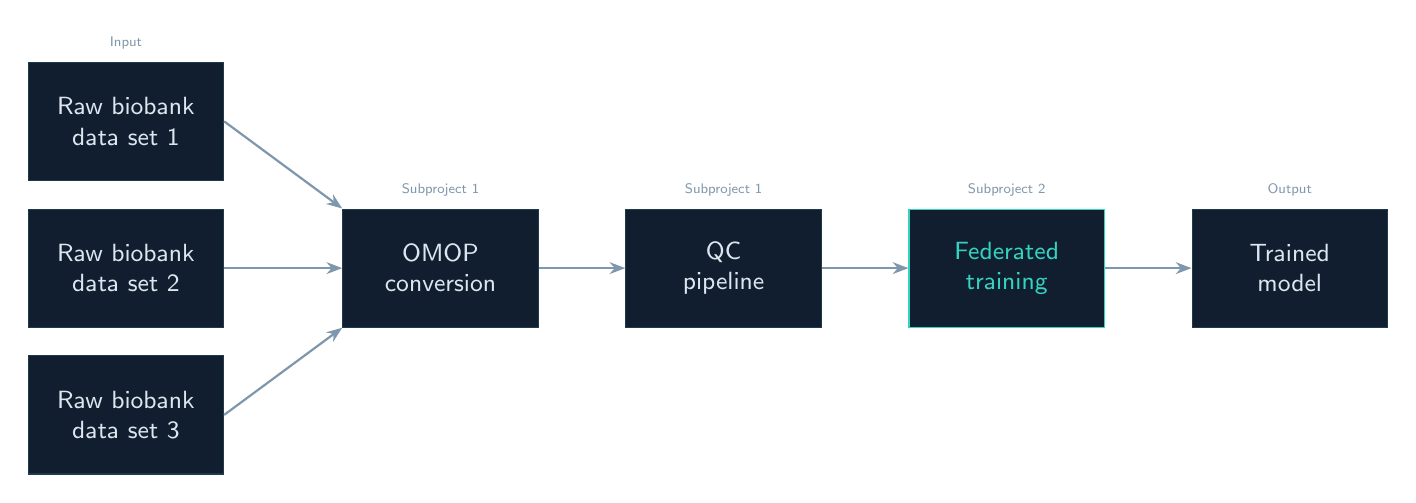
\begin{tikzpicture}[
      box/.style={draw=rulecol,fill=panel,text=fg,align=center,font=\small,
                  minimum height=1.5cm,text width=2.2cm,inner sep=4pt},
      hi/.style={box,draw=accent,text=accent},
      lbl/.style={font=\tiny,color=muted},
      arr/.style={-{Stealth[length=2mm]},draw=muted,thick}]

    \node[box] (in2) {Raw biobank\\data set 2};
    \node[box,above=0.35cm of in2] (in1) {Raw biobank\\data set 1};
    \node[box,below=0.35cm of in2] (in3) {Raw biobank\\data set 3};

    \node[box,right=1.5cm of in2] (conv) {OMOP\\conversion};
    \node[box,right=1.1cm of conv] (qc) {QC\\pipeline};
    \node[hi,right=1.1cm of qc] (fed) {Federated\\training};
    \node[box,right=1.1cm of fed] (out) {Trained\\model};

    \draw[arr] (in1.east) -- (conv.north west);
    \draw[arr] (in2.east) -- (conv.west);
    \draw[arr] (in3.east) -- (conv.south west);
    \draw[arr] (conv) -- (qc);
    \draw[arr] (qc) -- (fed);
    \draw[arr] (fed) -- (out);

    \node[lbl,above=1pt of conv] {Subproject 1};
    \node[lbl,above=1pt of qc] {Subproject 1};
    \node[lbl,above=1pt of fed] {Subproject 2};
    \node[lbl,above=1pt of out] {Output};
    \node[lbl,above=1pt of in1] {Input};
  \end{tikzpicture}

  \vspace{1.2em}
  {\color{muted}\small Every box exists. They are connected.}
  \note{This is the whole thing. Raw datasets in on the left, convert, quality
  control, federated training, trained model out. Every box in that diagram
  exists, and they are connected.}
\end{frame}

% ================================================ 3. SUBPROJECT 1 / WHY =====
\begin{frame}
  \frametitle{OMOP conversion \& quality control}
  \framesubtitle{Subproject 1}
  \vspace{1.0em}
  \begin{columns}[t]
    \begin{column}{0.46\textwidth}
      \colhead{The problem}
      \begin{itemize}
        \item Every biobank stores its data differently
        \item OMOP makes analysis portable across sites
        \item Status quo: hand-built ETL per source, months of work
      \end{itemize}
    \end{column}
    \begin{column}{0.46\textwidth}
      \colhead{Our approach}
      \begin{itemize}
        \item An agent skill that converts
        \item Not a script written for one dataset
        \item Scope: minimal table set, synthetic data, measurable
      \end{itemize}
    \end{column}
  \end{columns}
  \note{Why this is hard. Every biobank stores its data differently. OMOP is
  what makes analysis portable. Getting there today means a hand-built ETL per
  source, months of work. Our approach is an agent skill that converts, rather
  than a script written for one dataset.}
\end{frame}

% =========================================== 4. SUBPROJECT 1 / PIPELINE =====
\begin{frame}
  \frametitle{OMOP conversion \& quality control}
  \framesubtitle{Subproject 1}
  \vspace{0.8em}
  \begin{columns}[t]
    \begin{column}{0.48\textwidth}
      \colhead{Conversion pipeline}
      \begin{itemize}
        \item Profile the source: fields, codes, distributions
        \item Propose structural mapping: source field $\rightarrow$ OMOP field
        \item Propose vocabulary mapping: source code $\rightarrow$ standard concept
        \item \textbf{Clinical sign-off} before a mapping is accepted
        \item Run ETL: contracted tables, one directory per site
      \end{itemize}
    \end{column}
    \begin{column}{0.48\textwidth}
      \colhead{Quality control}
      \begin{itemize}
        \item Reference: published expert mappings (EHDEN, The Hyve)
        \item Expert mappings recovered, correctly and wrongly
        \item Share of records on \texttt{concept\_id = 0}
        \item Ten most frequent unmapped codes
        \item Output handed over via a fixed data contract
      \end{itemize}
    \end{column}
  \end{columns}
  \note{The first three steps are automated. Step four is deliberately a human,
  because a wrong but plausible concept is exactly what nobody catches later.
  Step five is plain code. Quality control measures against published expert
  mappings.}
\end{frame}

% ====================================== 5. SUBPROJECT 2 / IMPLEMENTATION ====
\begin{frame}
  \frametitle{Federated learning on OMOP data}
  \framesubtitle{Subproject 2}
  \vspace{0.6em}
  \begin{columns}[t]
    \begin{column}{0.48\textwidth}
      \colhead{Implementation}
      \begin{itemize}\small
        \item DuckDB enables lazy loading
        \item Time series stored as 3D sparse arrays: patients $\times$ concepts $\times$ time
        \item Custom PyTorch dataloader, validated on 5 Synthea OMOP cohorts
        \item \texttt{omopflare} exposes one API, integrates with NVFlare
      \end{itemize}
    \end{column}
    \begin{column}{0.48\textwidth}
      \colhead{Scope \& objective}
      \begin{itemize}\small
        \item Cox proportional hazards across simulated federated sites
        \item Goal is {\color{accent}end-to-end pipeline functionality}, not predictive performance
        \item Consumes OMOP output from subproject 1 directly
      \end{itemize}
    \end{column}
  \end{columns}

  \vspace{0.8em}
  \centering
  \figslot{fig_auroc_sites.png}{0.44\textwidth}{fig\_auroc\_sites.png\\
    Fragmenting a cohort costs a local model 10 AUROC points; federating recovers them}
  \hfill
  \figslot{fig_duckdb_scaling.png}{0.44\textwidth}{fig\_duckdb\_scaling.png\\
    Design matrix build stays sub-second to 50M rows}

  \note{The first problem is not the model, it is the data layout. Almost every
  cell is empty, so we store it sparse and read it lazily through DuckDB.
  Right: sub-second to fifty million rows. Left: split one cohort across
  sixteen sites and a local model loses about ten AUROC points, federated
  training recovers them.}
\end{frame}

% ================================================ 6. SUBPROJECT 2 / POC =====
\begin{frame}
  \frametitle{Federated learning on OMOP data}
  \framesubtitle{Subproject 2 $\cdot$ proof of concept on simulated data}
  \vspace{0.6em}
  \begin{columns}[t]
    \begin{column}{0.22\textwidth}
      \colhead{Biomarkers}
      {\small
      BMI\\ SBP\\ HbA1c\\ Glucose\\ Creatinine\\ eGFR}
    \end{column}
    \begin{column}{0.72\textwidth}
      \colhead{Model}
      \begin{itemize}\small
        \item Cox proportional hazards, 5-year survival
        \item Predictors: age and blood-based biomarkers
        \item Federation framework in place, single cohort for the first demo
        \item Nine federated rounds: C-index $\approx 0.71$, Brier score stable
      \end{itemize}
      \vspace{0.4em}
      \centering
      \figslot{fig_rounds.png}{0.62\textwidth}{fig\_rounds.png\\
        C-index and Brier score across federated rounds}
    \end{column}
  \end{columns}
  \note{Cox proportional hazards, five-year survival, age plus six blood
  biomarkers. Nine rounds, C-index around 0.71, Brier stable.}
\end{frame}

% =========================================== 7. SUBPROJECT 2 / COEFFS =======
\begin{frame}
  \frametitle{The coefficients point the right way}
  \framesubtitle{Subproject 2 $\cdot$ proof of concept on simulated data}
  \vspace{0.4em}
  \begin{columns}[c]
    \begin{column}{0.52\textwidth}
      \centering
      \figslot{fig_coefficients.png}{0.98\textwidth}{fig\_coefficients.png\\
        Log-hazard coefficients}
    \end{column}
    \begin{column}{0.42\textwidth}
      \begin{itemize}
        \item Age, HbA1c, systolic pressure and BMI raise the hazard
        \item eGFR lowers it
        \item {\color{accent}On synthetic data this is not biology}
        \item It shows the pipeline is wired correctly, end to end
      \end{itemize}
    \end{column}
  \end{columns}
  \note{The coefficients point the right way. On synthetic data that is not a
  biological finding. What it tells us is that the pipeline is wired correctly.}
\end{frame}

% ============================================================== 8. CLOSE ====
\begin{frame}[plain]
  \vspace{2.2em}
  \eyebrow{What we are claiming}
  \vspace{0.6em}

  {\color{fg}\fontsize{26}{32}\selectfont\bfseries
   A complete path from raw biobank data\\ to a federated model.}\par
  \vspace{1.0em}
  {\color{accent}\Large The data never left its site.}\par
  \vspace{2.0em}
  {\color{muted}\small Not predictive performance. Synthetic data throughout.
   Measurable at every step.}\par
  \vspace{1.6em}
  {\color{muted}\footnotesize
   \texttt{github.com/collaborativebioinformatics/Everything\_OMOP}}
  \note{Which is the claim. Not predictive performance. A complete path from
  raw biobank data to a federated model, and the data never left its site.}
\end{frame}

\end{document}
